\chapter{Documentação}
O objetivo da pesquisa é localizar pontos comuns entre usúarios portadores de afetividades negativas (stress, ansiedade e depressão) afim de caracterizar tais dimensões nesses perfis. Esse tipo de caracterização se asemelha muito com uma aprendizagem não supervisionada, logo, antes mesmo dessa caracterização é necessário mapearmos atributos que serão usados para isso fazendo-se necessário a identificação de usúarios com dimensões afetivas negativas primeiro.

Como observado, existem vários passos para conclusão desse projeto, nossa estrutura de processamento contára com um processo de mineração e dois processos de inteligencia artificial afim de gerar dois modelos lógicos. O primeiro modelo responsavel por inferir valores da EADS em um perfil, e o segundo, de predizer a partir de dados do perfil a chance de ter algum nivel de afetividade especifico.

O projeto por tras dessa pesquisa tem alguns outros pontos sociais envolvidos, que assim, tornam a área de atuação da pesquisa um pouco mais ampla, entretando nenhum desses pontos, exceto a utilização de profissionais capacidados para geração de alguns atributos em nossa base, impactam diretamentamente a \textit{performance} e por isso não serão detalhados. Logo essa documentação é voltada unicamente ao sistema que desenvolveremos.

Pode-se observar na figura 6, o sistema é divido em dois núcleos, o Dumont responsável por minerar e gerar toda nossa base de dados, e o 14BIS que será responsavel pelas Inteligencias Artificias. O aparente terceiro núcleo, na realidade, é simplesmente um banco de dados integrado gerado pelo APPA dentro do Dumont e que será consumido pelo 14BIS posteriormente.

\begin{figure}[H]
    \centering
    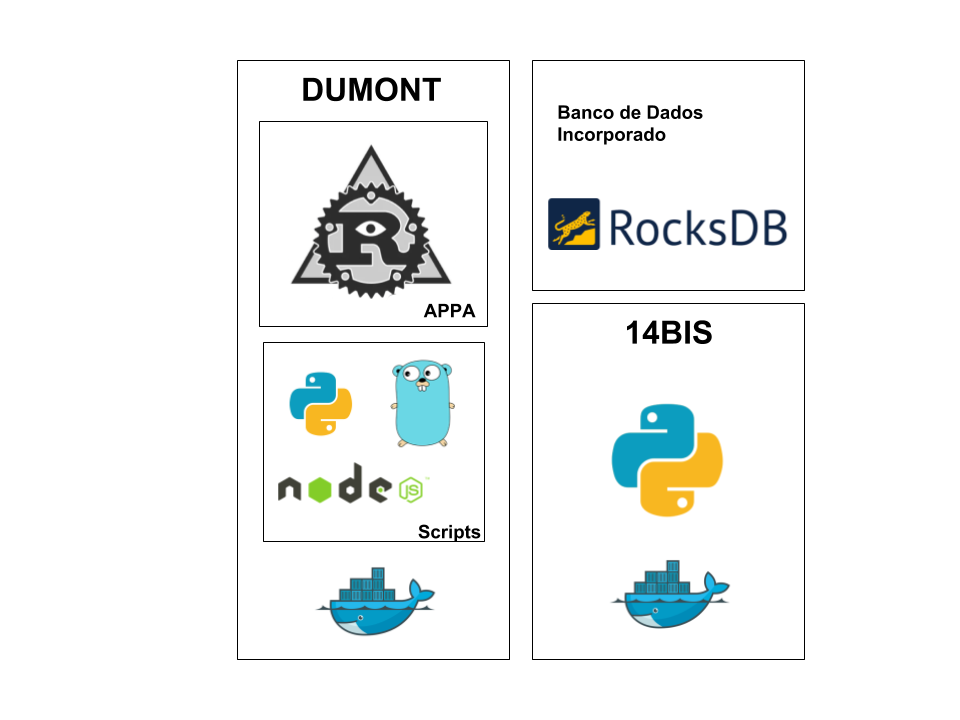
\includegraphics[width=.8\textwidth]{imagens/tecnologias.png}
    \caption{Desenho apresentando os núcleos do projeto}
    \label{fig:tecnologias}
\end{figure}

Existem basicamente 5 técnologias em evidencia:
\begin{itemize}
 \item Rust: Rust é uma linguagem altamente performatica, preza por custo zero em abstração, atua com excelencia em processamento paralelo e seu modelo de alocação de memória evita \textit{dataraces}\footnote{}
 \item Python: É a linguagem atual mais utilizada no mundo de Aprendizado de Máquina, sua simplicidade ja á torna simples de usar, porem, a quantidade de materiais, bibliotecas e artigos sobre o assunto á tornam nossa principal linguagem nesse projeto.
 \item Node/Javascript: Node é o interpretador que permite com que rodemos o Javascript (linguagem originalmente de browser no servidor). A linguagem tem um grande ganho com integrações e será utilizada para consumir recursos vindos de APIs.
 \item Go: Go se asemelha muito com Rust, porem, tem um ambiente menos burocratico devido a seus diferentes objetivos. Go será nossa escolha para qualquer processo que necessite muito recurso de processamento devido sua atual exploração dentro da area de IA.
 \item RocksDB: O RocksDB é um banco chave valor criado e distribuido gratuitamente pelo facebook. É um banco altamente performatico para leitura e escrita.
 \item Docker: Docker é uma ferramenta para infra-estrutura, será utilizado para rodar nossa aplicação em containers e facilitar nosso \textit{deploy}\footnote{}.
\end{itemize}

Existira uma sessão explicando o funcionamento do APPA, e como serão desenvolvidos os scripts que ele ira gerenciar, tanto quanto a parte explicativa sobre nossa Inteligencia Artificial, logo, nessa introdução os casos de uso serão tratados de forma sucinta. Se observar a figura 7, notara que o Dumont ira utilizar da API do twitter para coletar dados públicos, posteriormente esses dados serão processados e mutacionados a fim de gerar uma base de dados, por final essa base dados será salva em um banco embutido. Tanto o Dumont quanto o 14BIS irão consumir os dados salvos, porem é responsabilidade do 14BIS consumi-los a fim de treinar nossa IA para gerar nossos modelos lógicos.

\begin{figure}
    \centering
    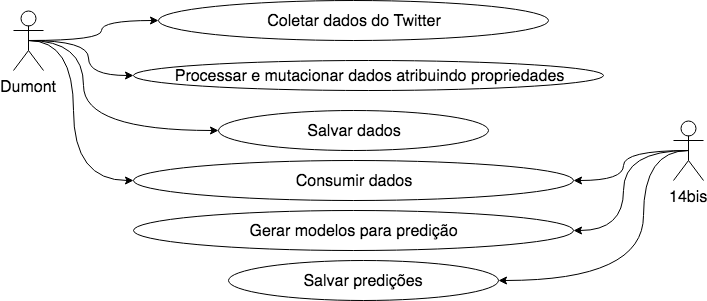
\includegraphics[width=.8\textwidth]{imagens/tcc_caso_de_uso.png}
    \caption{Diagrama de caso de uso do sistema}
    \label{fig:tcc_caso_de_uso}
\end{figure}

Para melhor entendimento a documentação será dividida em núcleos teóricos e práticos. Primeiramente será dado toda a descrição teórica sobre a escolha de atributos, e funcionamento das ferramentas que serão utilizadas no processo. Em seguida entratemos em núcleos mais práticos como a coleta e mineração, onde alem de explicar como rodar o Dumont, tambem serão explicados como e por que foram construidas essas partes do sistema. Como ja dito, a primeira etapa se consiste em entender nossos atributos.

\section{Engenharia de Atributos}
A escolha dos atributos, também intitulada popularmente como \textit{feature engineering}, é o ato mais importante durante a mineração de dados, por que é através desses atributos que as maquinas irão aprender. É válido destacar que essa sessão serve apenas para introduzir a razão dos atributos, seu detalhamento será dado durante a sua implementação.

O primeiro atributo relevante aqui é o sentimento. Já que será abordado dimensões afetivas negativas, o sentimento expressado por uma frase tem um grande impacto como atributo. Entretanto, o sentido em uma frase pode ser mais fácil de ser extraído em textos concisos, ou seja, normalizar os textos é necessário.

Um dos atributos utilizados aqui será o texto normalizado, para isso será utilizado o \textit{spacy}, uma biblioteca Python para remover palavras que oferecem apenas ruídos ao resultado. Além disso, também será tirada a arvore sintática, para que seja possível estabelecer padrões de discurso na IA, ou então, reconhecer certas palavras presentes em demais analises.

Uma vez observado os nossos atributos, seria necessário erguer um sistema capaz de realizar tarefas e persistir esses dados em algum banco de dados. Porém, será utilizado nessa pesquisa uma ferramenta para gerenciar tais tarefas.

\section{\textit{Application to Process and Produce Analytic Data (APPA)}}

Definir uma boa base de dados é o ponto mais critico durante a criação de uma inteligência supervisionada. O \textit{Application to Process and Produce Analytic Data} (APPA), ou, Aplicação para Processamento e Produção de Dados Analíticos, é um ferramenta criada capaz cadastrar tarefas, em qualquer linguagem e utilizar delas para coletar e processar esses dados afim de gerar uma base de conhecimento.

Explicando com mais detalhes, a figura \ref{fig:appa_eng} mostra o funcionamento da ferramenta. Existe uma arquivo chamado \textit{config.yml} que tem mapeado todas as tarefas e entidades de processamento. Essas tarefas podem ser escritas em qualquer linguagem de programação e algumas delas podem ser responsáveis por coletar dados, os scripts que são escritos com intuito de retornar dados para processamento são chamados coletores.

\begin{figure}
    \centering
    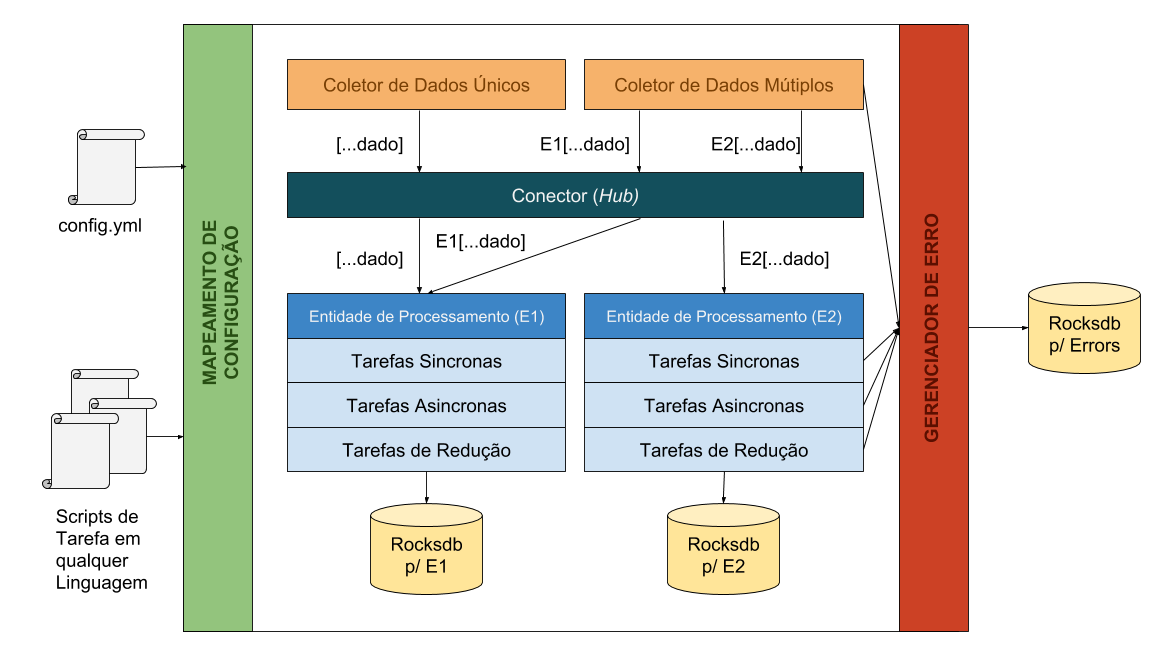
\includegraphics[width=.8\textwidth]{imagens/appa_eng.png}
    \caption{Diagrama demonstrando o funcionamento da ferramenta APPA}
    \label{fig:appa_eng}
\end{figure}

Um dado emitido por um coletor é marcado ou não por uma \textit{tag}, ou marcação, essa responsável por creditar qual coletor será responsável por processar. Por padrão um dado enviado sem destino é marcado com o simbolo \textit{underline}. Toda tarefa dentro do APPA é considerada uma tarefa com múltiplas saídas, logo, é possível enviar dados em lotes e tempo real para que o APPA processe dentro das entidades. 

Entidades de processamento, por sua vez, são compostas por coletores e tarefas de processamento. As tarefas de processamento podem ser síncronas ou assíncronas, ambas executam individualmente por unidade de dado, algo similar a uma linha de dados de um banco, a diferença é seu formato de execução, como o próprio nome fala as tarefas assíncronas não respeitam ordem de execução e são executadas paralelamente pelo processador. Alem disso existem as redutoras e/ou mapeadoras, consumiram todo o banco gerado após a execução das tarefas síncronas e assíncronas e retornara um novo estado para o banco total. Cada entidade gera seus dados em um banco incorporado isolado para os dados processados por elas.

Diferente de outras ferramentas, o processo de mineração nunca é interrompido. Qualquer erro que aconteça na aplicação é gerenciado por uma camada e registrado em um banco de erros, após isso o processamento segue para os demais dados.

\section{Coleta de Dados}
A coleta será feita utilizando a API publica do twitter, o link para a documentção é \url{https://developer.twitter.com/en/docs}. Será trabalhado no projeto duas entidades: Tweet e Usuário. O tweet é a entidade que representa a publicação do usuário, enquanto o usuário contém informações necessárias sobre o seu perfil.

Para que seja possível acessar a API é necessário criar uma conta de desenvolvimento e gerar o \textit{token} de acesso através do link \url{https://apps.twitter.com/app/new}. Com a chave em mãos é possível replicar o arquivo /collector/client/.env\_sample dentro do projeto Dumont para /collector/client/.env, e conforme demonstrado na figura \ref{fig:twitteropts}, completar os campos necessários.

\begin{figure}
    \centering
    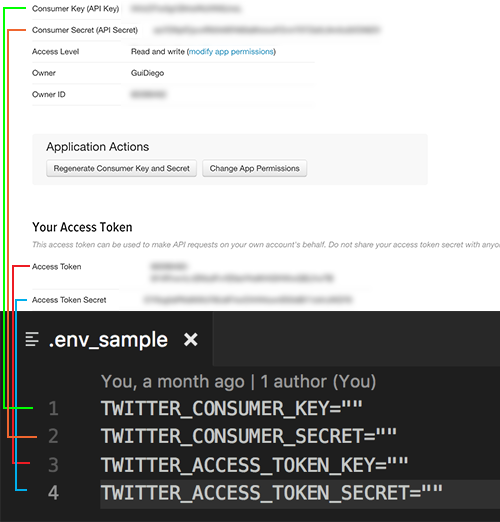
\includegraphics[width=.8\textwidth]{imagens/twitteropts.png}
    \caption{Diagrama demonstrando o funcionamento da ferramenta APPA}
    \label{fig:twitteropts}
\end{figure}

Para rodar basta executar o comando \textit{docker run -it --rm --name dumont -v \$"PWD":/usr/src/app -w /usr/src/app node:9 node collector/twitter.js}, e verá a saída de dados.

Uma vez configurado o coletor, ainda é necessário entender e configurar as outras tarefas para que o APPA funcione apropriadamente, logo, é necessário entender como essas entidades ficarão no final e quais as tarefas que realização essa manipulação.


% \section{Mineração de Dados}

